\documentclass[conference]{IEEEtran}
\usepackage{cite}
\usepackage{amsmath,amssymb,amsfonts}
\usepackage{graphicx}
\usepackage[caption=false,font=footnotesize]{subfig}
\usepackage{textcomp}
\usepackage{xcolor}
\usepackage{booktabs}
\captionsetup[subfloat]{justification=centering}
% Figures resolve from the repository's own data and results directories, so the
% document compiles anywhere the repository is checked out.
\graphicspath{{../data/processed/}{./figs/}{./figs/generated/}{./figs/visual_comparison/}}
\def\BibTeX{{\rm B\kern-.05em{\sc i\kern-.025em b}\kern-.08em
    T\kern-.1667em\lower.7ex\hbox{E}\kern-.125emX}}
\begin{document}

\title{Exploring Classical and Learning-Based Approaches to Image Compression}

\author{\IEEEauthorblockN{Leonardo Stefani}
\IEEEauthorblockA{Mid Sweden University\\
Sundsvall, Sweden \\
lest2502@student.miun.se}}

\maketitle

\begin{abstract}
Image-centric applications (streaming, healthcare, VR/AR) require codecs that balance bitrate and fidelity. This work benchmarks three standardised codecs (JPEG, JPEG2000, AVIF) against the Steered Mixture of Experts (SMoE) model on five 8-bit grayscale images, reporting rate, PSNR/SSIM, Spatial Information and encode time. Unlike quality-setting comparisons, every operating point is placed on a common rate axis in bits per pixel, which makes the codecs directly comparable. Classical codecs reach high fidelity at sub-second encodes across the full rate range. SMoE is behind on all three axes: at matched bitrate it trails the best classical codec by $8$--$27$~dB PSNR, it needs $8$--$211$ minutes per image rather than fractions of a second, and at its largest kernel budget the model itself costs up to $20.1$~bits per pixel---more than transmitting the uncompressed image.
\end{abstract}

\begin{IEEEkeywords}
JPEG, JPEG2000, AVIF, SMoE: Steered Mixture of Experts, PSNR: Peak Signal-to-Noise Ratio, SSIM: Structural Similarity Index, SI: Spatial Information, rate-distortion.\@
\end{IEEEkeywords}

\section{Introduction}
High-resolution imagery for virtual reality, live streaming, and mobile devices stresses storage and bandwidth. Classical codecs rely on fixed transforms and entropy coding, while recent machine learning approaches attempt to exploit richer spatial structure. This study takes three codec standards into consideration---JPEG, JPEG2000 and AVIF---and compares them to a learned compression method, the Steered Mixture of Experts (SMoE)~\cite{bochinski2018}. SMoE models images as adaptive Gaussian kernels aligned with edges, promising perceptual fidelity but imposing heavy computation.

The motivation is the rapid growth of visual data across streaming, healthcare, and mobile platforms, where storage and bandwidth pressures demand compression that preserves perceptual quality. Classical transform codecs are efficient but can struggle with complex structures; SMoE proposes an adaptive, context-aware alternative.

The goal is to compare classical codecs and SMoE under identical preprocessing, reporting rate, objective fidelity (PSNR/SSIM and Spatial Information) and elapsed time, consistent with prior comparative work~\cite{bochinski2018,bojkovic2001,sulema2010,gireesh2018,satone2017}.

\subsection{Problem Framing}
Classical codecs compress by transforming blocks (JPEG)~\cite{watson1994} or subbands (JPEG2000/AVIF), quantizing coefficients, and entropy coding \cite{sulema2010,adams2000}. SMoE instead treats compression as per-image regression: it learns a set of Gaussian experts whose weighted sum approximates the pixel field \cite{bochinski2018}. The research problem is to determine whether such adaptive models can deliver better rate-distortion performance without prohibitive computational cost, and whether they are practical replacements for established standards.

\subsection{Research Questions}
\begin{itemize}
    \item \textbf{RQ1}: How does SMoE perform on PSNR/SSIM compared to classical codecs (JPEG, JPEG2000, AVIF)?
    \item \textbf{RQ2}: What is the relationship between visual quality, compressed size and computational time?
    \item \textbf{RQ3}: Is SMoE computationally feasible compared to established codecs for practical deployment?
\end{itemize}

\subsection{Hypotheses}
\begin{itemize}
    \item Classical codecs will deliver near-lossless PSNR/SSIM at high qualities within sub-second encodes.
    \item SMoE will underperform on textured scenes and consume orders of magnitude more time per image, even at its best kernel budget.
\end{itemize}
Both were supported. A third result was not anticipated: SMoE is also uncompetitive on \emph{rate}, once rate is measured as the cost of transmitting the model.

\section{Related Work}
Classical codecs (JPEG, JPEG2000, AVIF) use hand-designed transforms and entropy coding to exploit spatial redundancy~\cite{bojkovic2001,sulema2010,gireesh2018,satone2017,adams2000,taubman2000}, with AVIF generally outperforming JPEG at similar bitrates \cite{sulema2010}. SMoE instead regresses pixel intensities with a steered Gaussian mixture, trained per image \cite{bochinski2018}. Prior surveys highlight the efficiency and maturity of classical standards~\cite{bojkovic2001,sulema2010,gireesh2018,satone2017}; broader surveys of learned compression \cite{jamil2023} note that per-image optimisation trades encode cost for adaptivity. PSNR and SSIM \cite{wang2004} remain common objective metrics despite imperfect perceptual alignment.

\section{Experimental Setup}

\subsection{Data}
Five 8-bit grayscale square images were used: \textit{Gradient} ($1280^2$), \textit{Grass} ($1274^2$), \textit{Mixed} ($2300^2$), \textit{Nature} ($1200^2$) and \textit{Sharp Edges} ($1486^2$), shown in Fig.~\ref{fig:fiveimagegrid}. The dataset size was constrained by SMoE's per-image training time; diversity of structure and texture was prioritized over scale. Inputs were squared and grayscaled to meet the requirements of the reference SMoE implementation, and all four codecs then operate on identical pixels.

\begin{figure}[t]
  \centering
  \subfloat[Gradient\label{fig:gradient}]{%
    \includegraphics[width=0.18\linewidth]{\detokenize{Gradient_sq_gray.png}}%
  }\hfill
  \subfloat[Grass\label{fig:grass}]{%
    \includegraphics[width=0.18\linewidth]{\detokenize{Grass_sq_gray.png}}%
  }\hfill
  \subfloat[Mixed\label{fig:mixed}]{%
    \includegraphics[width=0.18\linewidth]{\detokenize{Mixed_sq_gray.png}}%
  }\hfill
  \subfloat[Nature\label{fig:nature}]{%
    \includegraphics[width=0.18\linewidth]{\detokenize{Nature_sq_gray.png}}%
  }\hfill
  \subfloat[Sharp Edges\label{fig:sharpedges}]{%
    \includegraphics[width=0.18\linewidth]{\detokenize{SharpEdges_sq_gray.png}}%
  }
  \caption{Benchmark images used for the evaluation.}\label{fig:fiveimagegrid}
\end{figure}

\subsection{Codec Configuration}
JPEG was swept over quality factors $10$--$100$ with chroma subsampling disabled. JPEG2000 was swept using PSNR-targeted rate control ($28$--$60$~dB) plus a reversible, mathematically lossless setting. AVIF was swept over quality $10$--$100$ using \texttt{pillow-heif} at encoder speed~$6$. Because the sources are single-channel, all codecs encode grayscale natively; encoding grayscale as RGB inflates the compressed size by $16$--$73$\% and would bias the rate comparison.

SMoE was trained per image on $512\times512$ tiles with 64-pixel overlap and 100 iterations per tile, using Adam (TensorFlow~1.x compatibility mode) with $\ell_1$ sparsity on the gating weights. Reconstructions were feathered with a separable Hann window and reassembled. Three kernel budgets were run: $K \in \{16, 32, 96\}$ kernels per dimension, so $K^2$ kernels per tile before pruning.

\subsection{Metrics}
PSNR and SSIM were used for their practicality and broad applicability~\cite{sulema2010,gireesh2018}. SSIM uses the Gaussian $\sigma=1.5$ window of Wang et al.~\cite{wang2004}. To complement them, Spatial Information (SI) is computed as the standard deviation of the Sobel gradient magnitude (ITU-T P.910); higher SI indicates better preservation of structural detail.

Crucially, every operating point also records the \emph{rate}
\begin{equation}
    \mathrm{bpp} = \frac{8\,B}{W \times H},
\end{equation}
where $B$ is the encoded size in bytes. Quality settings are not comparable across codecs---a JPEG quality of $50$ and an AVIF quality of $50$ are unrelated operating points---so bpp is the only axis on which the four methods can be placed side by side.

\subsubsection{Measuring the SMoE rate}
For the classical codecs $B$ is the bitstream length. For SMoE the transmitted payload is the fitted model, not the decoded image. Each surviving kernel $j$ carries a gating weight $\pi_j$, a centre $\boldsymbol{\mu}_j \in \mathbb{R}^2$, a steering matrix $\mathbf{A}_j \in \mathbb{R}^{2\times2}$ with $\boldsymbol{\Sigma}_j^{-1} = \mathbf{A}_j^{\top}\mathbf{A}_j$, and expert parameters $(\boldsymbol{\gamma}_j, \nu_j)$, giving ten stored values per kernel. With $K_t$ kernels surviving $\ell_1$ pruning in tile $t$ and $b$ bits per value,
\begin{equation}
    \mathrm{bpp}_{\mathrm{SMoE}} = \frac{10\,b \sum_{t} K_t}{W \times H}.
    \label{eq:smoerate}
\end{equation}
The reference implementation stores \texttt{float32}, so $b=32$ is the measured rate. No quantisation or entropy coding of SMoE parameters is implemented, so this is the honest figure; an $8$-bit bound is also reported for context but is not achieved.

\subsection{Hardware and Timing}
SMoE training used a 16~GB NVIDIA Tesla P100 GPU; classical encodes used an Intel i7-1165G7 CPU, reported as the median of five runs after a warm-up. Timing for SMoE includes tiling, training and stitching; timing for the classical codecs covers encode only. The comparison therefore spans different hardware and should be read as an order-of-magnitude statement---which is sufficient at the observed $10^{4}$--$10^{5}\times$ gap.

\section{Results}

\subsection{Aggregate Quality}
Table~\ref{tab:aggregate} and Fig.~\ref{fig:aggregate} report min/mean/max PSNR and SSIM across all lossy operating points. Mathematically lossless points (JPEG2000 in reversible mode, and AVIF at its top setting on some content, where measured MSE is exactly zero and PSNR is unbounded) are excluded from the fidelity aggregates and reported separately; averaging an infinite value into a fidelity summary is meaningless, and substituting a large finite number would conceal the fact.

\begin{table}[h]
\centering
\begin{tabular}{lccccc}
\toprule
 & \textbf{Pts} & \textbf{PSNR} & \textbf{PSNR} & \textbf{SSIM} & \textbf{SSIM} \\
 & & \textbf{mean} & \textbf{std} & \textbf{mean} & \textbf{std} \\
\midrule
AVIF     & 45 & \textbf{42.81} & 9.15 & 0.965 & 0.067 \\
JPEG2000 & 45 & 42.67 & 9.60 & \textbf{0.967} & 0.046 \\
JPEG     & 50 & 41.48 & 9.77 & 0.958 & \textbf{0.045} \\
SMoE     & 14 & 29.66 & 6.86 & 0.859 & 0.172 \\
\bottomrule
\end{tabular}
\caption{Aggregate quality over all lossy operating points. Lossless points excluded.}
\label{tab:aggregate}
\end{table}

The three classical codecs are within $1.4$~dB of each other in mean PSNR, while SMoE trails the best by $13.2$~dB. SMoE also has by far the highest SSIM standard deviation ($0.172$ against $0.045$--$0.067$), indicating markedly less consistent behaviour across content types.

\begin{figure}[t]
\centering
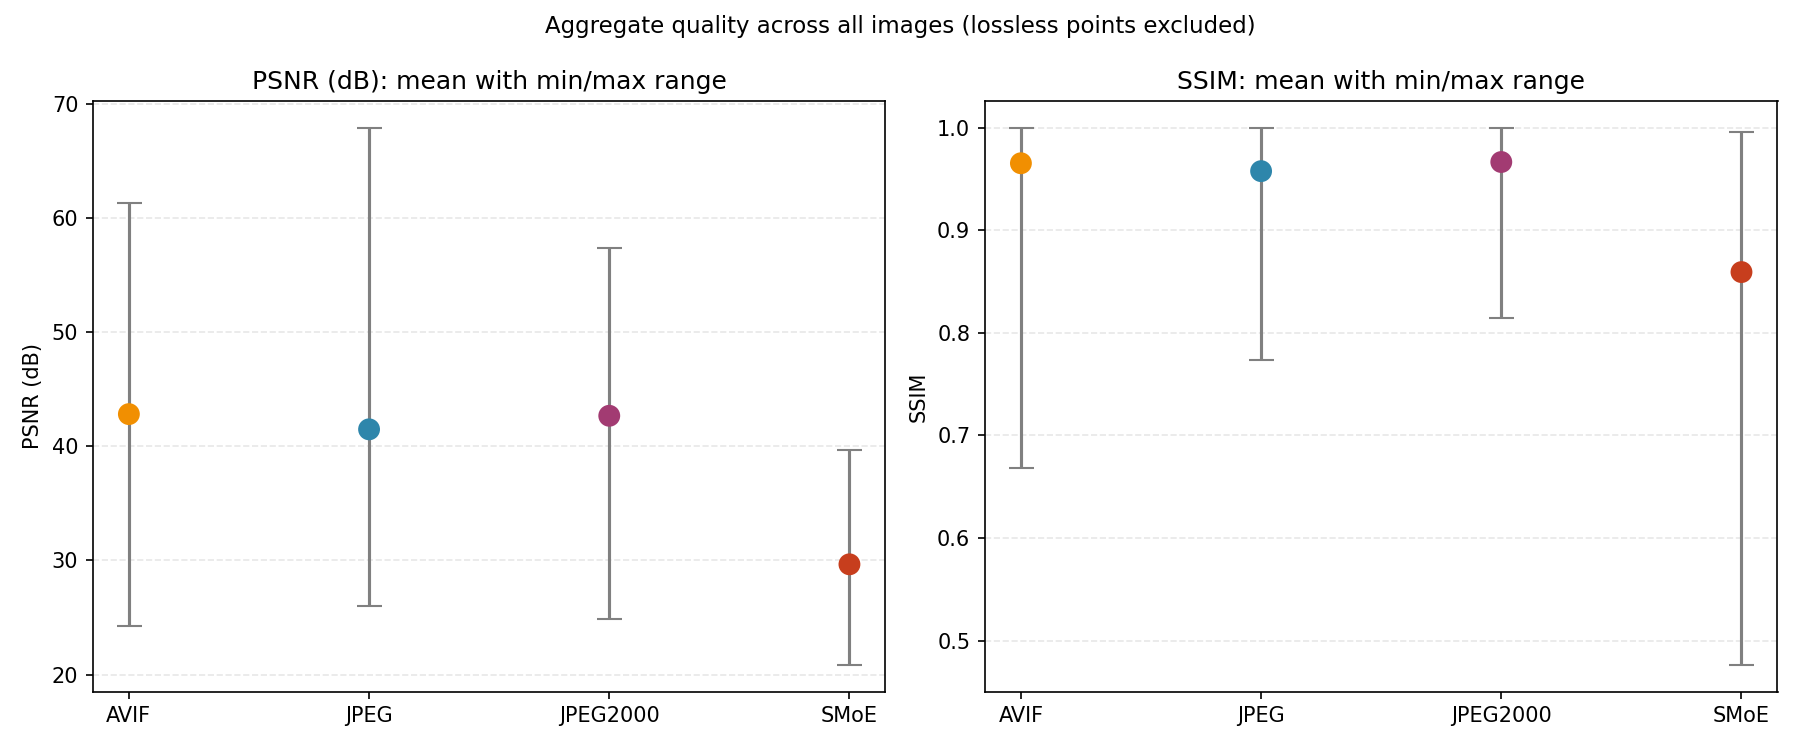
\includegraphics[width=\linewidth]{aggregate_quality.png}
\caption{Aggregate PSNR and SSIM (mean with min/max range) across all images. Classical codecs cluster together; SMoE sits well below on both metrics.}\label{fig:aggregate}
\end{figure}

\subsection{Rate-Distortion}
Fig.~\ref{fig:rd} plots PSNR against rate. The three classical curves cluster tightly, with AVIF and JPEG2000 leading JPEG at low and mid rates. SMoE lies far below all of them at every rate, and its highest-quality operating point falls to the \emph{right} of the $8$~bpp uncompressed reference: at $K=96$ the model costs $14.4$--$20.1$~bpp on four of the five images, so transmitting it is more expensive than sending the raw image, for a reconstruction of $25$--$40$~dB.

\begin{figure}[t]
\centering
\subfloat[\textit{Nature}]{\includegraphics[width=0.48\linewidth]{\detokenize{rd_psnr_Nature_sq_gray.png}}}\hfill
\subfloat[\textit{Grass}]{\includegraphics[width=0.48\linewidth]{\detokenize{rd_psnr_Grass_sq_gray.png}}}
\caption{Rate-distortion curves. The dotted vertical line marks the 8~bpp uncompressed reference. SMoE is below every classical curve across the whole rate range.}\label{fig:rd}
\end{figure}

Table~\ref{tab:matched} makes the comparison explicit by pairing each SMoE point with classical points within $\pm15$\% of the same bitrate. At matched rate SMoE is $8.4$--$26.5$~dB behind. The deficit is smallest on \textit{Nature}, whose fine photographic detail is hard for every codec at low rate, and largest on the textured and mixed content that edge-aware modelling was expected to favour.

\begin{table}[h]
\centering
\begin{tabular}{llcc l c}
\toprule
\textbf{Image} & \textbf{SMoE} & \textbf{bpp} & \textbf{PSNR} & \textbf{Best rival} & \textbf{Gap} \\
\midrule
Gradient   & $K{=}16$ & 0.45 & 39.56 & JPEG2000 & $-14.2$ \\
Grass      & $K{=}16$ & 0.45 & 22.09 & AVIF     & $-26.5$ \\
Mixed      & $K{=}16$ & 0.39 & 23.07 & AVIF     & $-25.7$ \\
Nature     & $K{=}16$ & 0.51 & 20.84 & AVIF     & $-8.4$ \\
Nature     & $K{=}32$ & 2.05 & 22.13 & AVIF     & $-18.9$ \\
\bottomrule
\end{tabular}
\caption{SMoE against the best classical codec at comparable rate ($\pm15$\% bpp). Gap in dB PSNR.}
\label{tab:matched}
\end{table}

\subsection{Time vs. Quality}
Fig.~\ref{fig:naturetime} plots PSNR against logarithmic encode time for \textit{Nature}. JPEG, JPEG2000 and AVIF achieve high quality in well under a second, while SMoE points appear far to the right with much lower PSNR. Table~\ref{tab:timing} gives the measured SMoE wall-clock times: from $7.7$ minutes at $K=16$ to $211$ minutes at $K=96$, against $0.04$--$2$~s for the classical encodes. The time penalty is not marginal---even the smallest kernel budget costs minutes per image.

\begin{figure}[t]
\centering
\includegraphics[width=0.85\linewidth]{\detokenize{time_psnr_Nature_sq_gray.png}}
\caption{\textit{Nature}: PSNR against encode time (log scale). SMoE is slower and lower-quality than all classical codecs. Note that SMoE ran on a GPU and the classical codecs on a CPU.}\label{fig:naturetime}
\end{figure}

\begin{table}[h]
\centering
\begin{tabular}{lccccc}
\toprule
\textbf{Budget} & \textbf{Grad.} & \textbf{Grass} & \textbf{Nature} & \textbf{Sharp} & \textbf{Mixed} \\
\midrule
$K{=}16$ & 7.9   & 7.7   & 7.7   & 13.7  & 21.5 \\
$K{=}32$ & 17.5  & 17.3  & 17.3  & 30.8  & 48.2 \\
$K{=}96$ & 120.9 & 113.0 & 106.5 & 211.0 & --- \\
\bottomrule
\end{tabular}
\caption{SMoE wall-clock time in minutes (tiling, training and stitching). The $K{=}96$ run for \textit{Mixed} did not complete.}
\label{tab:timing}
\end{table}

\subsection{Spatial Information}
Fig.~\ref{fig:si} reports SI against rate for \textit{Grass}. Classical codecs trace smooth, monotonic SI gains as rate rises. SMoE appears as sparse points at low SI, indicating it fails to preserve high-frequency structure. SI therefore reinforces the PSNR/SSIM conclusion: the gap is most visible on textured regions, where edge-aware modelling might have been expected to help.

\begin{figure}[t]
\centering
\includegraphics[width=0.85\linewidth]{\detokenize{si_Grass_sq_gray.png}}
\caption{Spatial Information against rate (\textit{Grass}). Classical codecs retain far more structural detail than SMoE at every bitrate.}\label{fig:si}
\end{figure}

\section{Research Ethics and Reproducibility}
The study uses grayscale synthetic patterns and natural photographs with no human-subject or personal data. All codecs share identical preprocessing and evaluation code, and PSNR/SSIM/SI are standard, well-documented metrics.

Reproducibility was treated as a first-class requirement. All figures and tables in this paper are generated from committed CSV files by scripts in the accompanying repository; no measurement is transcribed by hand. Metric implementations are unit-tested against \texttt{scikit-image} and agree to machine precision. Because codec output depends on the underlying \texttt{libjpeg}, \texttt{OpenJPEG} and \texttt{libaom} builds, dependency versions are pinned and the environment used for the committed results is recorded.

An audit of an earlier version of this work identified a substantive error: the SMoE ``file size'' had been taken as the byte size of the reconstructed PNG---the decoder \emph{output}---rather than the transmitted model. That inflated SMoE's apparent rate efficiency and led to the incorrect conclusion that it compressed competitively. Equation~\eqref{eq:smoerate} replaces it. The audit also found that two result directories had been mislabelled with the wrong kernel budget, and that two configurations had produced byte-identical reconstructions; the affected data has been relabelled by verified kernel count and the duplicate excluded. Both the audit and the corrections are documented in the repository.

\section{Discussion}
Across images a consistent pattern emerges: SMoE is the weakest performer on PSNR, SSIM, SI and rate for every content type tested. Classical codecs maintain high fidelity across all content, indicating robustness to scene statistics---which matters for real deployments, where input diversity is the norm.

\subsection{Visual Comparison}
Fig.~\ref{fig:visual} shows \textit{Nature} at the highest quality setting for each method. JPEG, JPEG2000 and AVIF are visually indistinguishable from the source. SMoE shows softened textures and faint tile seams, consistent with its lower PSNR/SSIM and SI. The difference is clearest in high-contrast regions such as the tree in the upper right.

\begin{figure}[t]
\centering
\subfloat[JPEG Q100]{\includegraphics[width=0.46\linewidth]{\detokenize{Nature_sq_gray_JPEG_Q100.jpg}}}\hfill
\subfloat[JPEG2000 lossless]{\includegraphics[width=0.46\linewidth]{\detokenize{Nature_sq_gray_Q100_converted.png}}}\\[2pt]
\subfloat[AVIF Q100]{\includegraphics[width=0.46\linewidth]{\detokenize{Nature_sq_gray_Q100_avif.png}}}\hfill
\subfloat[SMoE $K{=}96$]{\includegraphics[width=0.46\linewidth]{\detokenize{Nature_sq_gray_reconstructed.png}}}
\caption{Highest-quality reconstructions of \textit{Nature}. The classical codecs are visually lossless; SMoE blurs fine detail.}\label{fig:visual}
\end{figure}

\subsection{Limitations}
Five images buy structural diversity, not statistical power. Only three kernel budgets were run, leaving a gap between $K=32$ and $K=96$, and the $K=96$ run for \textit{Mixed} did not complete. SMoE and the classical codecs were timed on different hardware. Most importantly, no quantisation or entropy coding of SMoE parameters was implemented: the rates in Fig.~\ref{fig:rd} are what the reference implementation produces, and a purpose-built SMoE codec with parameter quantisation and an entropy coder would do better than the $\texttt{float32}$ figures reported here. Even the optimistic $8$-bit bound, however, leaves SMoE well behind at matched quality.

\subsection{Future Work}
Extending to colour images, perceptual metrics, variable kernel budgets per tile, and parameter quantisation with entropy coding are the immediate next steps. The last of these is the one that would most change the conclusions: it is the difference between measuring a research prototype and measuring a codec.

\section{Conclusion}
Classical codecs outperform SMoE on fidelity, rate and speed. At matched bitrate SMoE trails the best classical codec by $8$--$27$~dB; at its largest kernel budget the model costs more bits than the uncompressed image; and it needs tens to hundreds of minutes per image against fractions of a second. No configuration was found in which SMoE surpasses the classical baselines.

From a deployment standpoint, AVIF provides the best default, offering the strongest rate-distortion performance across content types. JPEG remains useful as a lowest-common-denominator format and a fast preview option. JPEG2000's progressive decoding and mathematically lossless mode suit archival tasks, though ecosystem support is weaker. SMoE is not competitive for production encoding in its current form, but it demonstrates the value of explicit edge modelling and may serve as a research scaffold for hybrid learned/wavelet methods.

\subsection{Research Question Outcomes}
\textbf{RQ1}: SMoE does not outperform classical codecs on PSNR, SSIM or SI. It trails on aggregate quality (Table~\ref{tab:aggregate}) and at every matched rate (Table~\ref{tab:matched}).

\textbf{RQ2}: Quality, rate and time all increase together, but at sharply different rates per codec. For the classical codecs, quality rises steeply with modest rate increases. For SMoE, both rate and time grow far faster than quality: moving from $K=32$ to $K=96$ multiplies the rate by roughly $8\times$ and the time by $6\times$ for gains of $2$--$6$~dB. SMoE is not competitive on any of the three axes.

\textbf{RQ3}: SMoE is not computationally feasible relative to established codecs. Fig.~\ref{fig:naturetime} shows orders-of-magnitude slower encodes for lower quality.

\subsection{Computational Considerations}
The cost gap is rooted in algorithmic design: classical codecs apply a fixed transform and lightweight entropy coding, while SMoE trains a fresh model per tile by gradient descent. Tiling multiplies this cost and adds blending overhead. Classical codecs also benefit from decades of optimisation and hardware acceleration. Any deployment demanding scale, interactivity or low latency therefore favours classical codecs by several orders of magnitude.

\subsection{Practical Implications}
Within this evaluation, SMoE fails the efficiency criterion (minutes to hours per image), the quality criterion (PSNR/SSIM and SI well below mid-quality classical settings) and the rate criterion (up to $20$~bpp, above the uncompressed reference). Prior work on classical codecs~\cite{bojkovic2001,satone2017} reinforces their practicality. This means:
\begin{itemize}
    \item For interactive or batch pipelines, classical codecs remain the only viable choice.
    \item SMoE requires parameter quantisation, entropy coding, and radical acceleration through fewer kernels, fewer iterations, distillation or pruning before it merits practical consideration.
\end{itemize}

\begin{thebibliography}{00}
\bibitem{bochinski2018} E.~Bochinski, R.~Jongebloed, M.~Tok, and T.~Sikora, ``Regularized gradient descent training of steered mixture of experts for sparse image representation'', in \emph{Proc. IEEE Int. Conf. Image Process. (ICIP)}, Athens, Greece, Oct. 2018.
\bibitem{bojkovic2001} Z.~Bojkovic and D.~Milovanovic, ``Advanced image compression techniques: comparative functionalities and performances'', in \emph{Proc. TELSIKS}, Nis, Yugoslavia, 2001, pp.~439--444~vol.~2, doi: 10.1109/TELSKS.2001.955815.
\bibitem{sulema2010} Y.~Sulema and S.~E.~Kahou, ``Image compression: Comparative analysis of basic algorithms'', in \emph{Proc. EWDTS}, St.~Petersburg, Russia, 2010, pp.~534--537, doi: 10.1109/EWDTS.2010.5742106.
\bibitem{gireesh2018} H.~R.~Gireesh and L.~Rangaiah, ``A survey on performance of various image compression techniques'', in \emph{Proc. ICEECCOT}, Mysuru, India, 2018, pp.~1233--1238, doi: 10.1109/ICEECCOT43722.2018.9001522.
\bibitem{satone2017} K.~N.~Satone, A.~S.~Deshmukh, and P.~B.~Ulhe, ``A review of image compression techniques'', in \emph{Proc. ICECA}, Coimbatore, India, 2017, pp.~97--101, doi: 10.1109/ICECA.2017.8203651.
\bibitem{watson1994} A.~B.~Watson, ``Image Compression Using the Discrete Cosine Transform'', \emph{Mathematica Journal}, vol.~4, no.~1, pp.~81--88, 1994.
\bibitem{adams2000} M.~D.~Adams and F.~Kossentini, ``Reversible integer-to-integer wavelet transforms for image compression: Performance evaluation and analysis'', \emph{IEEE Trans. Image Processing}, vol.~9, no.~6, pp.~1010--1024, 2000.
\bibitem{taubman2000} D.~Taubman, ``High performance scalable image compression with EBCOT'', \emph{IEEE Trans. Image Processing}, vol.~9, no.~7, 2000.
\bibitem{wang2004} Z.~Wang, A.~C.~Bovik, H.~R.~Sheikh, and E.~P.~Simoncelli, ``Image quality assessment: from error visibility to structural similarity'', \emph{IEEE Trans. Image Processing}, vol.~13, no.~4, pp.~600--612, 2004.
\bibitem{jamil2023} S.~Jamil, Md.~J.~Piran, M.~U.~Rahman, and O.-J.~Kwon, ``Learning-driven lossy image compression: A comprehensive survey'', \emph{Engineering Applications of Artificial Intelligence}, vol.~123, art.~106361, Aug. 2023, doi: 10.1016/j.engappai.2023.106361.
\end{thebibliography}

\end{document}
